\documentclass{article}
\usepackage[utf8]{inputenc}
\usepackage{amsmath}
\usepackage{amsfonts}
\usepackage{graphicx}
\usepackage{float}
\usepackage{caption}
\usepackage{subfigure}

\title{Computational Economics PS2}
\author{Saa}
\date{December 2022 (Updated. Jan 2024)}

\begin{document}
	
	\maketitle
	
	\section{Setting}
	
	Solve a stochastic growth model:
	\begin{equation}
		\begin{aligned}
			&\max \mathbb{E} \sum\limits_{t=0}^\infty \beta \frac{c_t^{1-\gamma}}{1-\gamma} \\
			&s.t. \quad \begin{array}{r@{\quad}r@{}l@{\quad}l}
				&Y_t &=exp(z_t)K_t^\alpha  \\
				&C_t + K_{t+1} &=Y_t + (1-\delta)K_t\\
				&z_{t+1} &= \rho z_t +e_{t+1}
			\end{array}
		\end{aligned}
	\end{equation}
	where $e_t\sim N(0, \sigma_{e})$ are i.i.d.
	
	The corresponding dynamic programming problem is:
	\begin{equation}
		\begin{aligned}
			&\max  V(k_t, z_t) = \frac{c_t^{1-\gamma}}{1-\gamma} +\beta \mathbb{E}_{z_t} V(k_{t+1}, z_{t+1})\\
			&s.t. \quad \begin{array}{r@{\quad}r@{}l@{\quad}l}
				&Y_t &=exp(z_t)K_t^\alpha  \\
				&C_t + K_{t+1} &=Y_t + (1-\delta)K_t\\
				&z_{t+1} &= \rho z_t +e_{t+1}
			\end{array}
		\end{aligned}
	\end{equation}
	where $K_t,z_t$ are state variables and $c_t, k_{t+1}$ are control variables.
	
	The steady state are:
	\begin{gather}
		k_{ss} = [\frac{1}{\alpha}(\frac{1}{\beta} - 1 + \delta)] ^{\frac{1}{\alpha - 1}}\\
		y_{ss} = k_{ss}^\alpha =  [\frac{1}{\alpha}(\frac{1}{\beta} - 1 + \delta)] ^{\frac{\alpha}{\alpha - 1}}\\
		c_{ss} = y_{ss} - \delta k_{ss} = [\frac{1}{\alpha}(\frac{1}{\beta} - 1 + \delta)] ^{\frac{\alpha}{\alpha - 1}} - \delta [\frac{1}{\alpha}(\frac{1}{\beta} - 1 + \delta)] ^{\frac{1}{\alpha - 1}}
	\end{gather}
	
	\section{Numerical Results}
	
	The value of the parameters are displayed in Table \ref{tab:param}.
	I use Tauchen method to approximate AR(1) process with grid number 5 and $m=3$.
	All the methods solve the problem in the range $[(1-width)*k_{ss},(1+width)*k_{ss}]$ with $n_k$ grids inside.
	\begin{table}[H]
		\centering
		\begin{tabular}{|c|c|}
			parameter & value \\ \hline
			$\gamma$ & 2\\
			$\alpha$ & 0.36\\
			$\beta$ & 0.99\\
			$\delta$ & 0.025\\
			$\rho$ & 0.95\\
			$\sigma_e$ & 0.007\\
			$n_k$ & 400\\
			$n_z$ & 5\\
			$m$ & 3\\
			$tol$ & 1e-5\\
			$width$ & 20\%
		\end{tabular}
		\caption{Parameters}
		\label{tab:param}
	\end{table}
	
	\subsection{Value Function Iteration}
	
	\subsubsection{Difference between Grid Numbers}
	
	First, it takes more time to do VFI with more grids.
	$n_k=200$, VFI takes 26.19s.
	$n_k=400$, VFI takes 60.70s.
	
	Second, VFI with more grids solves the model more accurately.
	Figure \ref{fig:nk} is the graph of the solved $K'-K$ for different $n_k$.
	We can see that the kink in VFI $n_k=200$ is larger.
	\begin{figure}[H]
		\centering
		\subfigure[$n_k=200$]{
			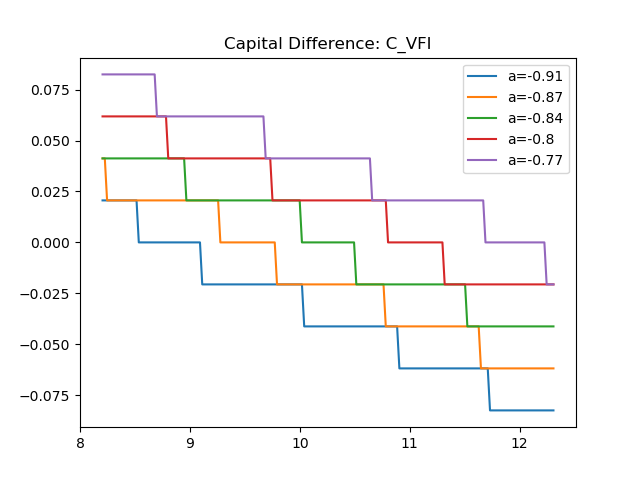
\includegraphics[width=0.45\textwidth]{../figures/problem_set_2/C_KDiff.png}
		}
		\subfigure[$n_k=400$]{
			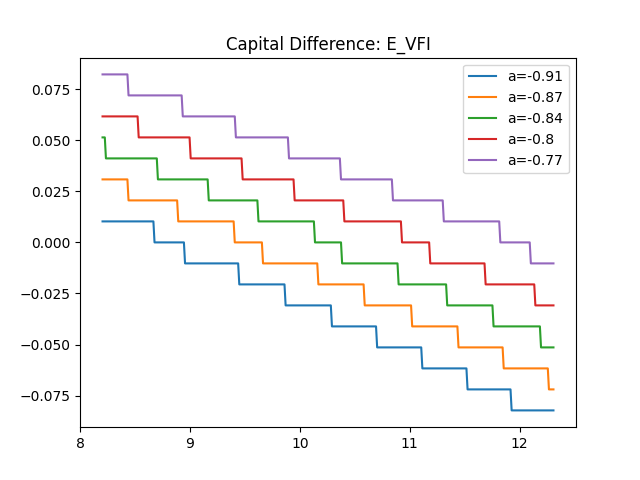
\includegraphics[width=0.45\textwidth]{../figures/problem_set_2/E_KDiff.png}
		}
		\caption{$K'-K$ for VFI with different $n_k$}
		\label{fig:nk}
	\end{figure}
	
	\subsubsection{Property of Value and Policy Function}
	
	\begin{figure}[H]
		\centering
		\subfigure[Value Function $V_z(K)$]{
			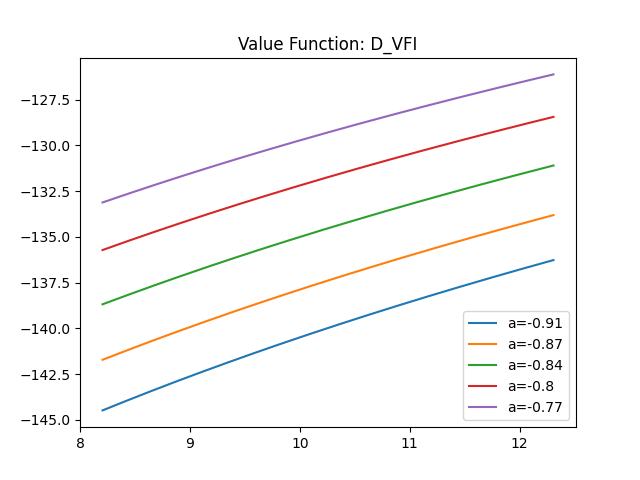
\includegraphics[width=0.3\textwidth]{../figures/problem_set_2/D_ValueFunc.png}
		}
		\subfigure[1st Derivative $V_z'(K)$]{
			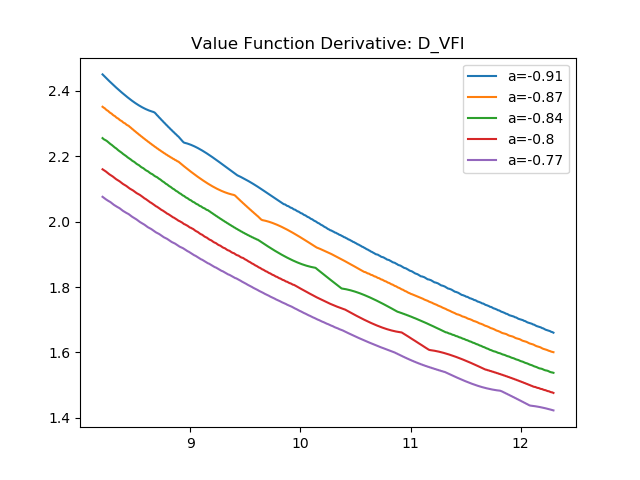
\includegraphics[width=0.3\textwidth]{../figures/problem_set_2/D_ValueFuncD.png}
		}
		\subfigure[2nd Derivative $V_z''(K)$]{
			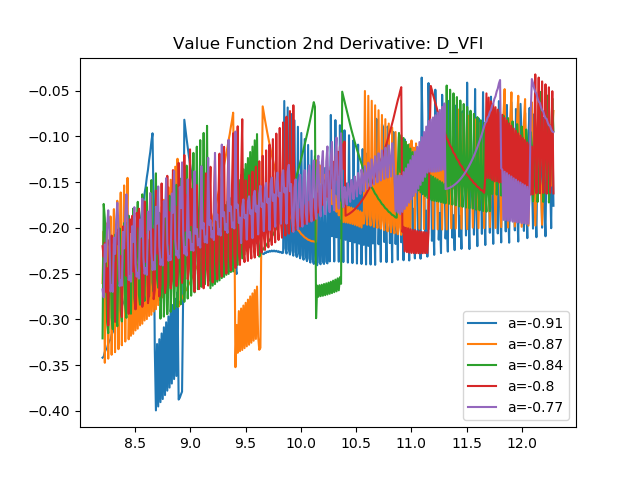
\includegraphics[width=0.3\textwidth]{../figures/problem_set_2/D_ValueFunc2D.png}
		}
		\caption{Value Function and its derivatives: VFI}
		\label{fig:vfunc_VFI}
	\end{figure}
	
	Figure \ref{fig:vfunc_VFI} is the value Function and its derivatives when $n_k=400$.
	The 1st derivative is greater than 0, and the 2nd derivative is less than 0.
	So value function is strictly increasing and concave.
	
	\begin{figure}[H]
		\centering
		\subfigure[Policy Function $K'_z(K)$]{
			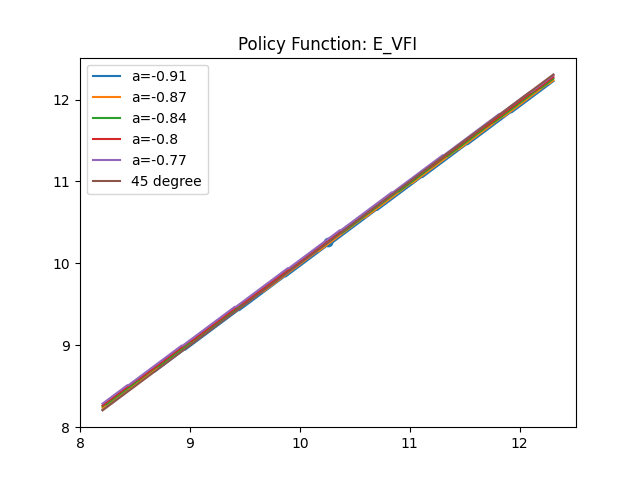
\includegraphics[width=0.3\textwidth]{../figures/problem_set_2/E_PolicyFunc.png}
		}
		\subfigure[1st Derivative $K'_z{}'(K)$]{
			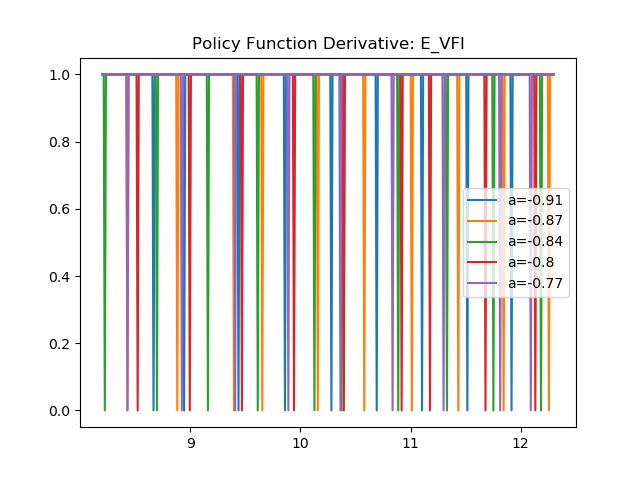
\includegraphics[width=0.3\textwidth]{../figures/problem_set_2/E_PolicyFuncD.png}
		}
		\subfigure[2nd Derivative $K'_z{}''(K)$]{
			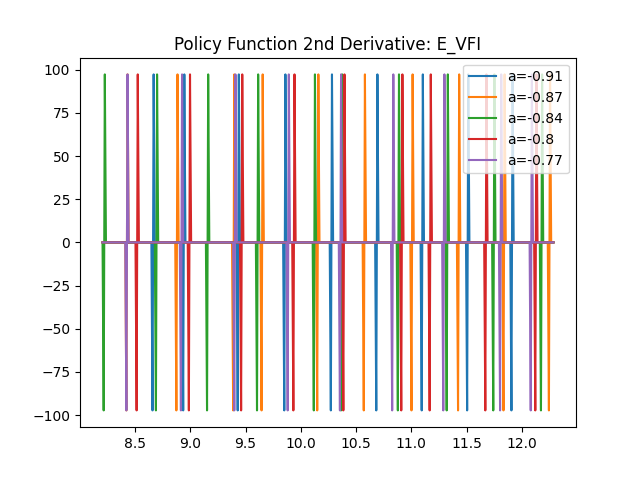
\includegraphics[width=0.3\textwidth]{../figures/problem_set_2/E_PolicyFunc2D.png}
		}
		\caption{Policy Function and its derivatives: VFI}
		\label{fig:pfunc_VFI}
	\end{figure}
	Figure \ref{fig:pfunc_VFI} is the policy Function and its derivatives when $n_k=400$.
	The 1st derivative is greater than 0.
	So policy function is increasing but not concave.
	
	\begin{figure}[H]
		\centering
		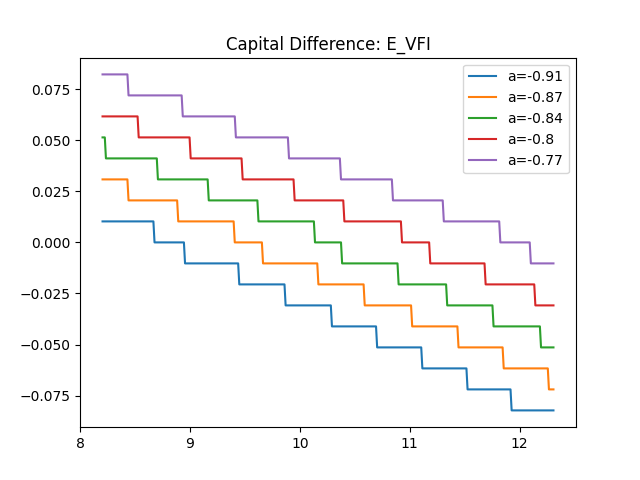
\includegraphics[width=0.8\textwidth]{../figures/problem_set_2/E_KDiff.png}
		\caption{Change in Decision Rule: VFI}
		\label{fig:dk_VFI}
	\end{figure}
	Figure \ref{fig:dk_VFI} is $K'(k,z)-K$.
	We can see that there is a lot of kinks.
	The discrete policy set in VFI may be a reason for these kinks.
	The precision of VFI is heavily limited by the width of grids.
	
	\subsubsection{Euler Error}
	
	\begin{figure}[H]
		\centering
		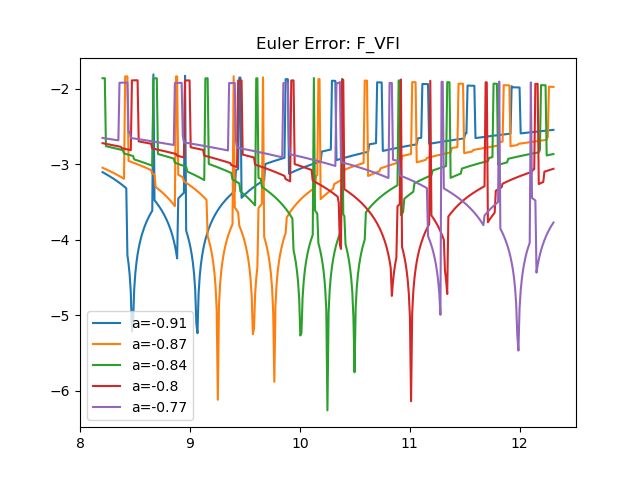
\includegraphics[width=0.8\textwidth]{../figures/problem_set_2/F_EulerErr.png}
		\caption{Euler Error: VFI}
		\label{fig:euler_VFI}
	\end{figure}
	Figure \ref{fig:euler_VFI} is the graph of Euler Equation Error $\epsilon(K,z)$, which is defined as:
	\begin{equation}
		\epsilon(K,z)=1-\frac{1}{c}u'^{-1}\left\{\ \beta\mathbb{E}_{z} [u'(c')(\alpha exp(z') K'^{\alpha -1 } +1 -\delta)] \right\}
	\end{equation}
	And the min, max, mean of Euler error are showed in Table \ref{tab:euler_VFI}.
	\begin{table}[H]
		\centering
		\begin{tabular}{|cccc|}
\hline
index & mean & min & max\\
-0.91 & -3.011 & -5.237 & -1.807\\
-0.87 & -3.164 & -6.12 & -1.831\\
-0.84 & -3.224 & -6.261 & -1.856\\
-0.8 & -3.194 & -6.14 & -1.875\\
-0.77 & -3.068 & -5.468 & -1.903\\
\hline
\end{tabular}


		\caption{Euler Equation Error of VFI}
		\label{tab:euler_VFI}
	\end{table}
	
	We will discuss all the simulation results at the end.
	
	\subsection{VFI Acceleration}
	
	Howard Policy Iteration takes 48.86s when $nh=5, nv=20$, and take 28.40s when $nh=20,nv=10$.
	HPI is faster than VFI.
	It becomes faster when $nh/nv$ increases.
	Figure \ref{fig:hpi} is the policy function of VFI and HPI.
	\begin{figure}[H]
		\centering
		\subfigure[VFI]{
			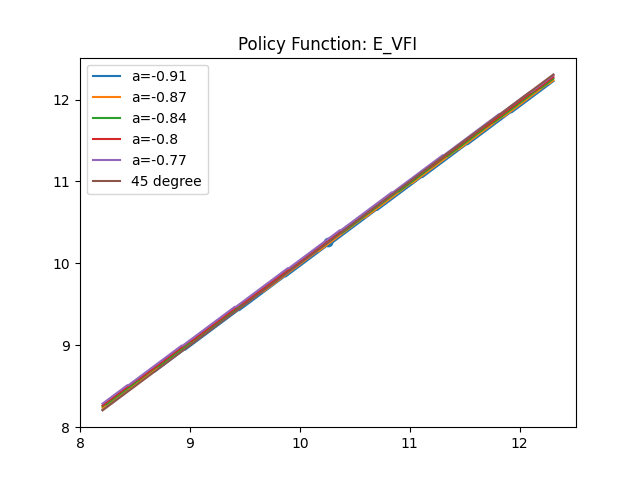
\includegraphics[width=0.45\textwidth]{../figures/problem_set_2/E_PolicyFunc.png}
		}
		\subfigure[HPI]{
			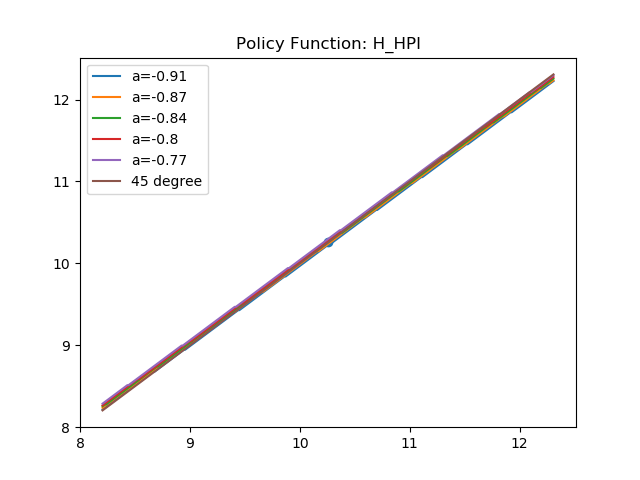
\includegraphics[width=0.45\textwidth]{../figures/problem_set_2/H_PolicyFunc.png}
		}
		\caption{Policy Function of VFI and HPI}
		\label{fig:hpi}
	\end{figure}
	
	McQueen Perteus error bound takes 23.06s.
	It's faster than the previous solutions.
	
	\subsection{Continuous Approximation}
	
	I use Chebyshev Polynomials to interpolate the value function and solve the policy function by numerically maximizing $u+\beta V$.
	With MQP and HPI $nh=20, nv=10$, it takes 1016.35s to converge.
	
	\begin{figure}[H]
		\centering
		\subfigure[Value Function $V_z(K)$]{
			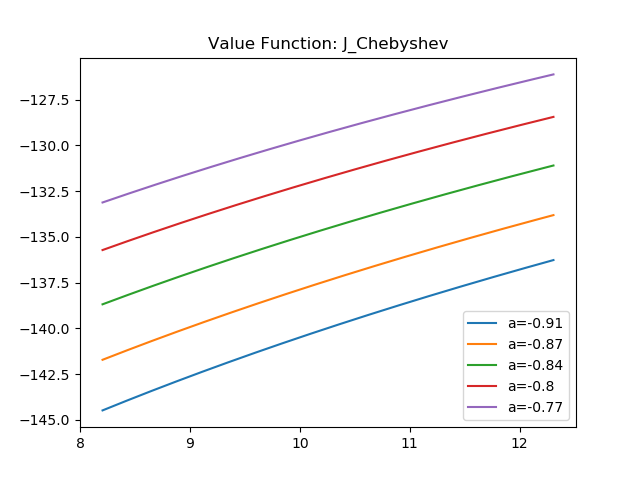
\includegraphics[width=0.3\textwidth]{../figures/problem_set_2/J_ValueFunc.png}
		}
		\subfigure[1st Derivative $V_z'(K)$]{
			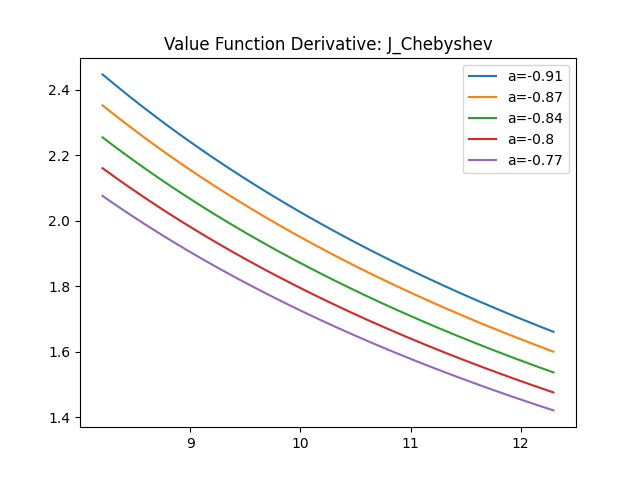
\includegraphics[width=0.3\textwidth]{../figures/problem_set_2/J_ValueFuncD.png}
		}
		\subfigure[2nd Derivative $V_z''(K)$]{
			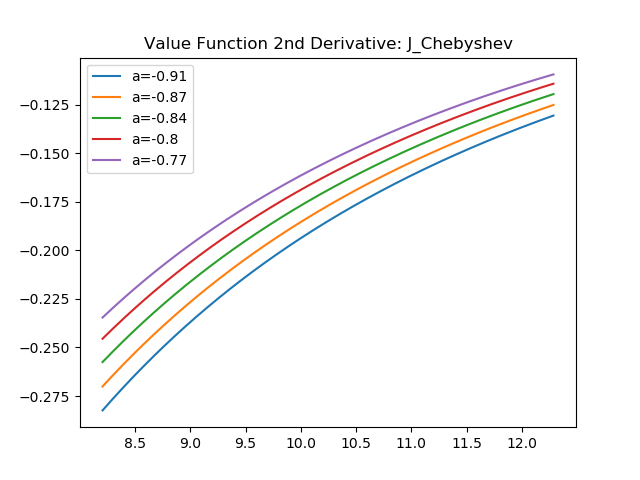
\includegraphics[width=0.3\textwidth]{../figures/problem_set_2/J_ValueFunc2D.png}
		}
		\caption{Value Function and its derivatives: VFI and Interpolation}
		\label{fig:vfunc_Che}
	\end{figure}
	
	Figure \ref{fig:vfunc_Che} is the value function.
	We can see the value function is still increasing and concave.
	
	\begin{figure}[H]
		\centering
		\subfigure[Policy Function $K'_z(K)$]{
			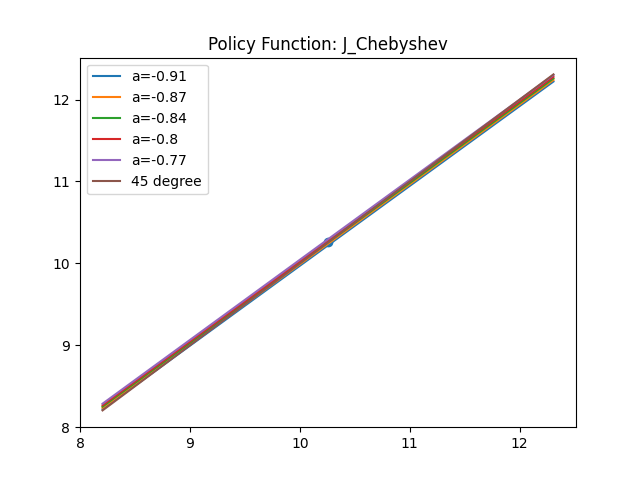
\includegraphics[width=0.3\textwidth]{../figures/problem_set_2/J_PolicyFunc.png}
		}
		\subfigure[1st Derivative $K'_z{}'(K)$]{
			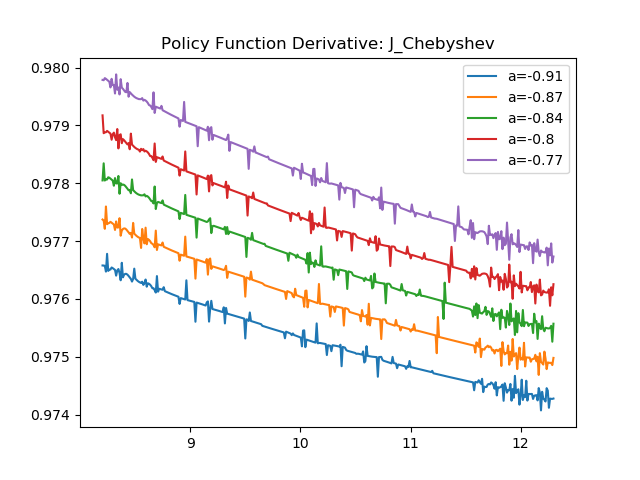
\includegraphics[width=0.3\textwidth]{../figures/problem_set_2/J_PolicyFuncD.png}
		}
		\subfigure[2nd Derivative $K'_z{}''(K)$]{
			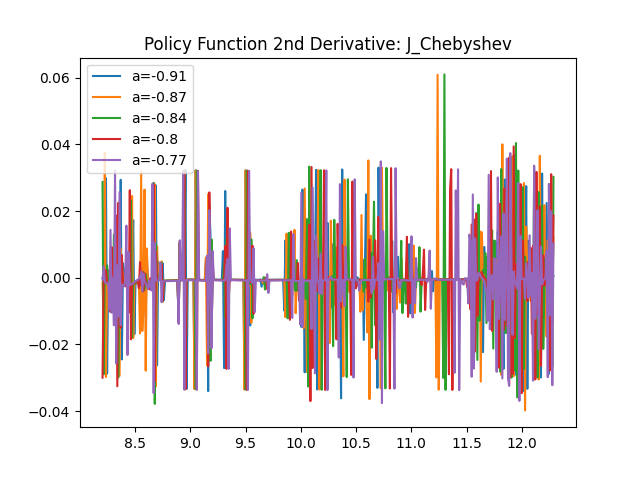
\includegraphics[width=0.3\textwidth]{../figures/problem_set_2/J_PolicyFunc2D.png}
		}
		\caption{Policy Function and its derivatives: VFI and Interpolation}
		\label{fig:pfunc_Che}
	\end{figure}
	
	Figure \ref{fig:pfunc_Che} is the policy function.
	We can see the policy function is still increasing but not concave.
	
	\begin{figure}[H]
		\centering
		\subfigure[VFI]{
			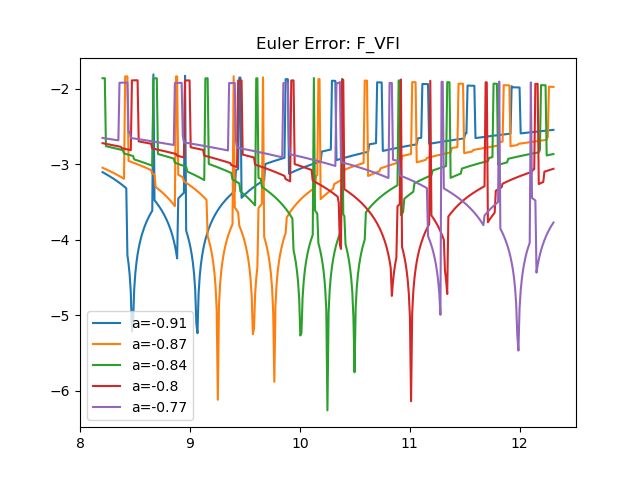
\includegraphics[width=0.45\textwidth]{../figures/problem_set_2/F_EulerErr.png}
		}
		\subfigure[VFI and Interpolation]{
			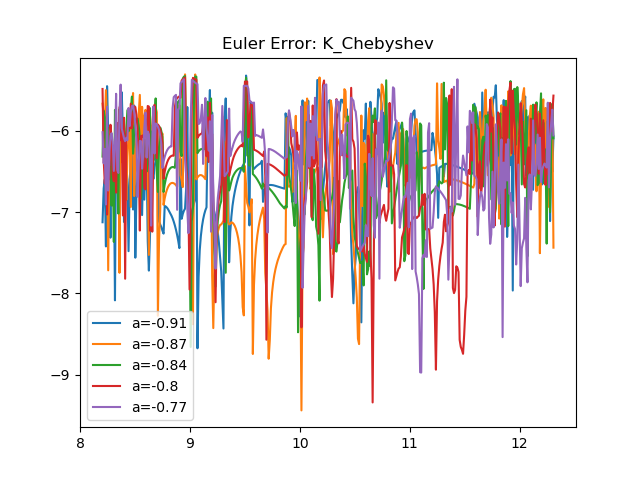
\includegraphics[width=0.45\textwidth]{../figures/problem_set_2/K_EulerErr.png}
		}
		\caption{Euler error of VFI and Interpolation}
		\label{fig:err_che}
	\end{figure}
	Figure \ref{fig:err_che} is the Euler errors of the two methods.
	We can see the Euler errors decrease a lot if the policy function is continuous.
	And Table \ref{tab:err_che} are their mean, min, and max.
	\begin{table}[H]
		\centering
		\begin{tabular}{|cccc|}
\hline
index & mean & min & max\\
-0.91 & -6.426 & -8.675 & -5.32\\
-0.87 & -6.534 & -9.591 & -5.306\\
-0.84 & -6.511 & -8.656 & -5.327\\
-0.8 & -6.523 & -9.314 & -5.344\\
-0.77 & -6.384 & -8.972 & -5.365\\
\hline
\end{tabular}


		\caption{Euler Error of VFI and Interpolation}
		\label{tab:err_che}
	\end{table}
	
	\subsection{Simulation Results}
	
	I first do simulation with different TFP series, but find that the moments and distribution cannot be compared.
	The moments are in Table \ref{tab:mom}.
	\begin{table}[H]
		\centering
		\begin{tabular}{|cccccc|}
\hline
index & VFI & Chebyshev Approximation & modified PEA & EGM & Real\\
sigma y & 0.0427 & 0.0441 & 0.0441 & 0.0435 & 1.8\\
sigma c & 0.0297 & 0.0299 & 0.0299 & 0.0298 & 1.3\\
sigma i & 0.0138 & 0.0147 & 0.0147 & 0.0141 & 5.1\\
corr(y, c) & 0.9915 & 0.9949 & 0.9948 & 0.9952 & 0.739\\
corr(y, i) & 0.9602 & 0.9785 & 0.9785 & 0.9785 & 0.714\\
corr(c, i) & 0.9157 & 0.9525 & 0.9525 & 0.9537 & -100.0\\
mean(k) & 10.1186 & 10.0912 & 10.0933 & 10.0844 & -100.0\\
mean(c) & 0.7334 & 0.7332 & 0.7333 & 0.7331 & -100.0\\
mean(y) & 0.9856 & 0.9846 & 0.9847 & 0.9844 & -100.0\\
mean(i) & 0.2522 & 0.2513 & 0.2514 & 0.2512 & -100.0\\
autocorr(y) & 0.9946 & 0.995 & 0.995 & 0.9948 & -100.0\\
autocorr(c) & 0.9973 & 0.9976 & 0.9976 & 0.9974 & -100.0\\
autocorr(i) & 0.9791 & 0.987 & 0.987 & 0.987 & -100.0\\
autocorr(a) & 0.9863 & 0.9863 & 0.9863 & 0.9863 & -100.0\\
\hline
\end{tabular}


		\caption{Simulation Moments: Different TFP Process}
		\label{tab:mom}
	\end{table}
	
	But from the above table we can see that the 4 series all show that the autocorrelation of TFP is larger than 0.95.
	Therefore, the Tauchen approximation of the AR(1) process is not good.
	
	\begin{figure}[H]
		\centering
		\subfigure[$K_t$]{
			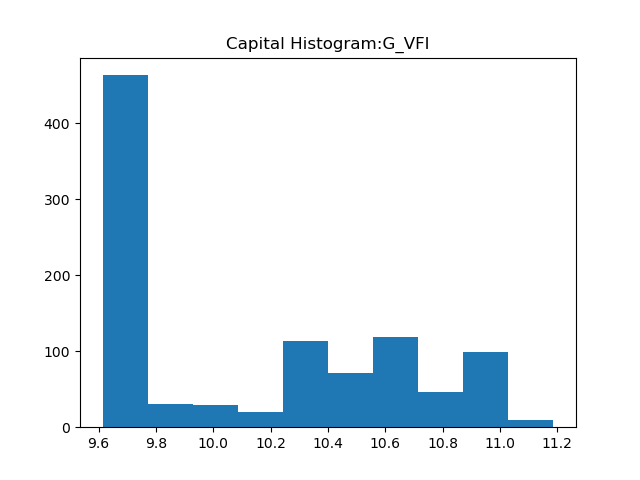
\includegraphics[width=0.45\textwidth]{../figures/problem_set_2/G_VFI_KHist.png}
		}
		\subfigure[$I_t/K_t$]{
			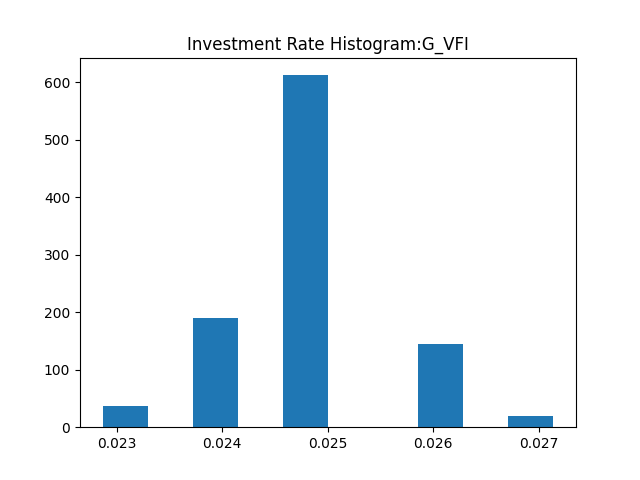
\includegraphics[width=0.45\textwidth]{../figures/problem_set_2/G_VFI_IRHist.png}
		}
		\caption{Histogram of Capital and Investment Rate: VFI}
		\label{fig:hist_VFI}
	\end{figure}
	
	\begin{figure}[H]
		\centering
		\subfigure[$K_t$]{
			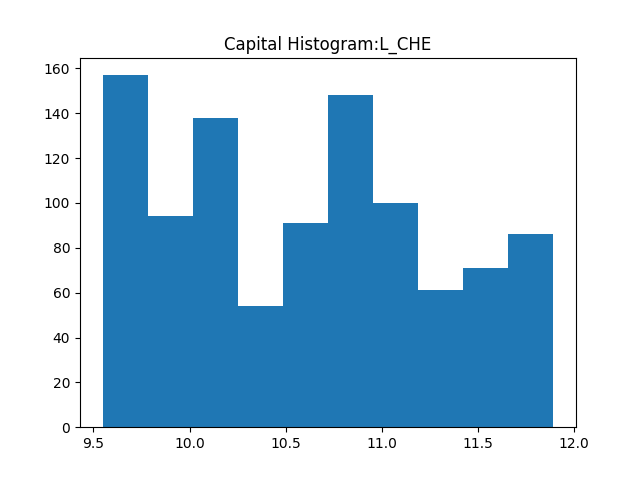
\includegraphics[width=0.45\textwidth]{../figures/problem_set_2/L_CHE_KHist.png}
		}
		\subfigure[$I_t/K_t$]{
			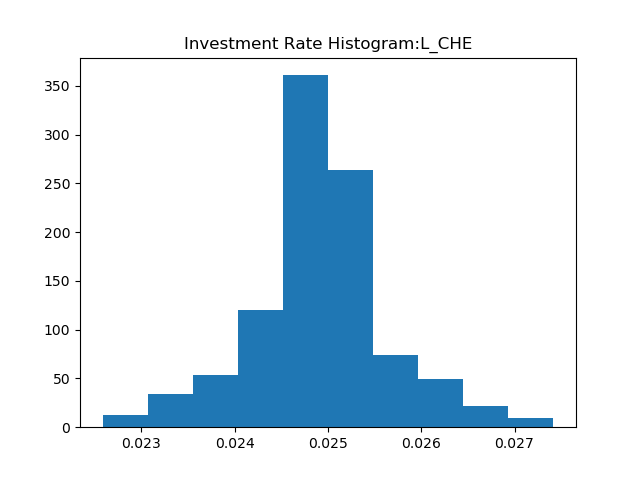
\includegraphics[width=0.45\textwidth]{../figures/problem_set_2/L_CHE_IRHist.png}
		}
		\caption{Histogram of Capital and Investment Rate: VFI \& Interp}
		\label{fig:hist_CHE}
	\end{figure}
	
	\begin{figure}[H]
		\centering
		\subfigure[$K_t$]{
			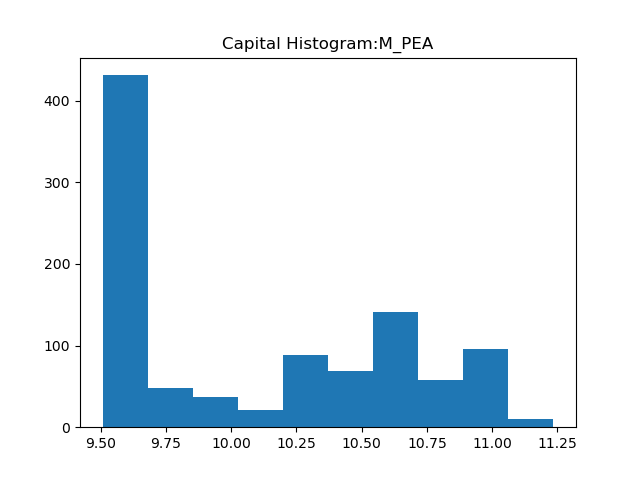
\includegraphics[width=0.45\textwidth]{../figures/problem_set_2/M_PEA_KHist.png}
		}
		\subfigure[$I_t/K_t$]{
			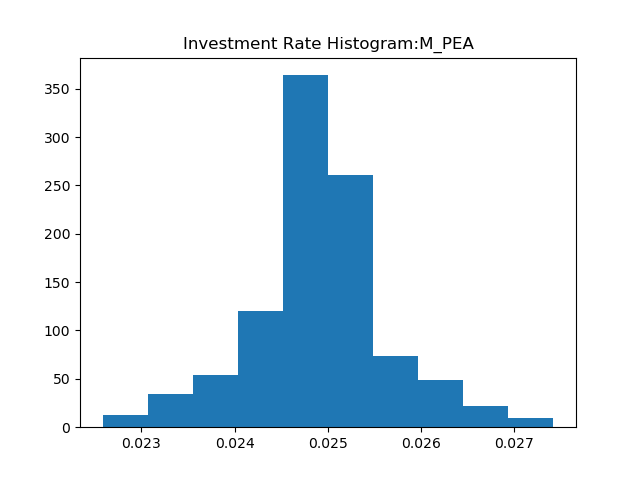
\includegraphics[width=0.45\textwidth]{../figures/problem_set_2/M_PEA_IRHist.png}
		}
		\caption{Histogram of Capital and Investment Rate: PEA}
		\label{fig:hist_PEA}
	\end{figure}
	
	\begin{figure}[H]
		\centering
		\subfigure[$K_t$]{
			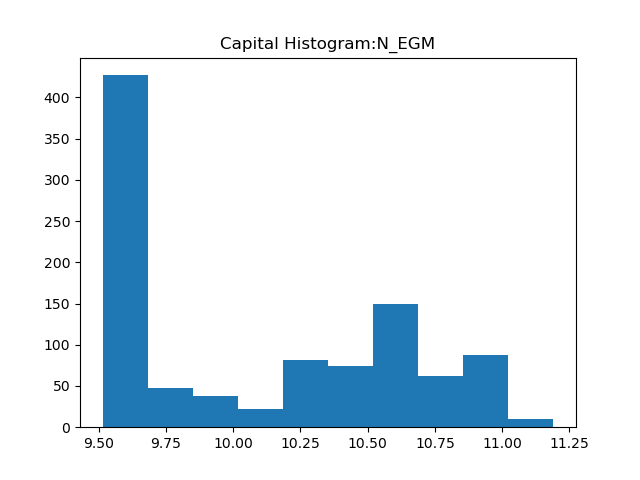
\includegraphics[width=0.45\textwidth]{../figures/problem_set_2/N_EGM_KHist.png}
		}
		\subfigure[$I_t/K_t$]{
			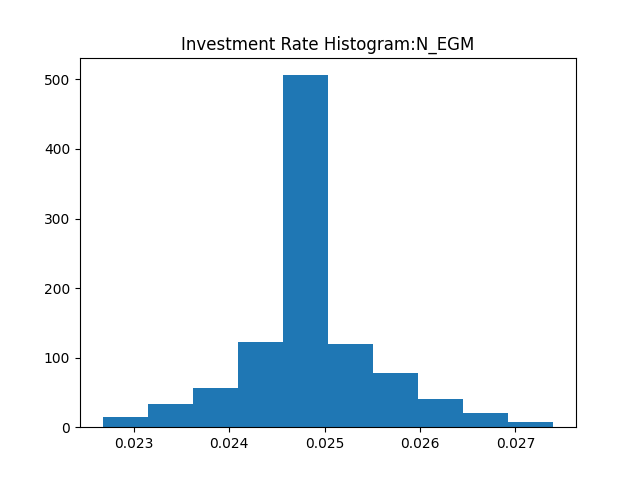
\includegraphics[width=0.45\textwidth]{../figures/problem_set_2/N_EGM_IRHist.png}
		}
		\caption{Histogram of Capital and Investment Rate: EGM}
		\label{fig:hist_EGM}
	\end{figure}
	Figure \ref{fig:hist_VFI}, \ref{fig:hist_CHE}, \ref{fig:hist_PEA}, \ref{fig:hist_EGM} are the histograms of capital and investment rate of VFI, VFI \& Interp, PEA, EGM, respectively.
	
	We can see that both two variables' distribution is centralized.
	The distribution of VFI is discrete because its policy set is discrete.
	Also, the Investment rate has smaller variation than capital.
	The distribution of VFI \& Interp and modified PEA is alike.
	The distribution of EGM is slightly different from the other two algorithms.
	
	\begin{table}[H]
		\centering
		\begin{tabular}{|cccccc|}
			\hline
			moment & VFI & VFI \& Interp & modified PEA & EGM & Real\\
			sigma y & 0.0427 & 0.0441 & 0.0441 & 0.0435 & 0.018\\
			sigma c & 0.0297 & 0.0299 & 0.0299 & 0.0298 & 0.0096\\
			sigma i & 0.0138 & 0.0147 & 0.0147 & 0.0141 & 0.0072\\
			corr(y, c) & 0.9915 & 0.9949 & 0.9948 & 0.9952 & 0.739\\
			corr(y, i) & 0.9602 & 0.9785 & 0.9785 & 0.9785 & 0.714\\
			corr(c, i) & 0.9157 & 0.9525 & 0.9525 & 0.9537 & -\\
			mean(k) & 10.1186 & 10.0912 & 10.0933 & 10.0844 & 10\\
			mean(c) & 0.7334 & 0.7332 & 0.7333 & 0.7331 & 0.843\\
			mean(y) & 0.9856 & 0.9846 & 0.9847 & 0.9844 & 1\\
			mean(i) & 0.2522 & 0.2513 & 0.2514 & 0.2512 & 0.142\\
			autocorr(y) & 0.9946 & 0.995 & 0.995 & 0.9948 & 0.84\\
			autocorr(c) & 0.9973 & 0.9976 & 0.9976 & 0.9974 & -\\
			autocorr(i) & 0.9791 & 0.987 & 0.987 & 0.987 & -\\
			autocorr(a) & 0.9863 & 0.9863 & 0.9863 & 0.9863 & 0.95\\
			\hline
		\end{tabular}
		\caption{Simulation Moments: the Same TFP Process}
		\label{tab:mom_same}
	\end{table}
	
	The simulated moments also verify the above conclusion.
	The moments of VFI \& Interp and modified PEA are close, while the VFI moments largely deviate from the other three algorithm.
	
	The real moments are estimated by Hodrick and Prescott 1997 JMCB paper except mean(k).
	The capital output ratio is taken from Doblin, C.P., 1991. Capital stock and capital output ratios: A comparison between the United States, United Kingdom and the Federal Republic of Germany.
	
	For the standard deviation, the model is less volatile than the real data.
	The correlation and autocorrelation are overestimated, which may result from the large autocorrelation of TFP.
	
	I define consumption as the sum of consumption and government spending.
	However, there may be some part of government spending can be categorized as investment.
	This may explain the high investment share of the model.
	
	Overall, I think the performance of the model can be improved by a better approximation of the TFP process.
\end{document}
